% ============================================================
% 4. Experimental Design
% ============================================================
\section{Experimental Design}
\label{sec:experiments}

\subsection{Task Suite}

The task suite consists of eight scenario tasks, each a natural-language
requirement written as an application scenario plus absolute numeric
criteria (Table~\ref{tab:tasks}). The scenarios span the design landscape
deliberately: a sedan (performance plus thermal safety), grid storage
(cycle life plus low temperature), power tools (rate plus power), extreme
cold (low temperature plus volumetric density), a flagship vehicle (extreme
energy density), a smartphone (volumetric ceiling plus a strict temperature
red line plus a voltage plateau), a hybrid vehicle (high-temperature aging
plus nail penetration), and a drone (specific energy plus a mass ceiling).
Across the eight tasks, fourteen distinct metric types are checked, and
all criteria of a task are AND-judged: a design must satisfy every clause
of its target to be ``achieved.''

Three design choices deserve emphasis. First, the tasks carry no constraint
declarations beyond the metrics: nothing states which variables are adjustable,
which chemistry to use, or where the baseline sits. Undeclared items are
interpreted in the widest sense under the workflow rules, with the derivation
recorded---this is what forces the agent to make the design-space decisions
itself. Second, every number in every task is absolute; no relative-baseline
phrasing appears, so an agent cannot redefine the reference it measures
against. Third, the tasks are heterogeneous in where their binding
constraint lives: T1, T4, and T8 are solvable inside a structural space
(thickness, porosity, mass), while T2, T3, T5, T6, and T7 require material,
formulation, or transport variables---the distinction on which the comparison
with the Bayesian baseline turns.

The target quantities are defined on standard cell models from the cited
literature. Plating is judged on the negative-electrode potential against
Li/Li$^+$, written as the sum of the equilibrium potential and the kinetic
overpotential \cite{arora1999plating, ren2018plating}:
\begin{equation}
\label{eq:phi}
\phi_{a} = U_a + \eta_c.
\end{equation}
The SEI criterion reads a state variable of the degradation model, whose
growth law supplies the coating variable that T2 and T6 exploit
\cite{peled1979sei, okane2022pccp}:
\begin{equation}
\label{eq:sei}
\frac{d\delta}{dt} = k_{\mathrm{SEI}},
\end{equation}
where $k_{\mathrm{SEI}}$ is exactly the parameter the electrode-modification
bridge adjusts. The thermal-runaway trigger for the overcharge and
nail-penetration criteria is the three-side-reaction energy balance
\cite{wang2012thermalrunaway}:
\begin{equation}
\label{eq:tr}
m c_p \frac{dT}{dt} = \sum_k \Delta H_k r_k(T) - hA\,(T - T_{\mathrm{amb}}),
\end{equation}
with $\text{triggered}$ iff the trajectory crosses the runaway onset; the
cooling coefficient $h$ is the thermal-management variable. Criterion values are model-relative (an SEI limit reads the state variable
of a specific degradation model, a plateau reads a specific OCP set) so
cross-system comparisons are made only within the same model. The scenario
anchoring (which production
specification each task draws from, and how each threshold was calibrated
from the underlying parameter sets) is documented in the supplementary
materials; each threshold is the anchoring parameter set's baseline value
for that criterion shifted by a fixed increment (e.g., $+20\%$ energy
density over the baseline configuration, a $5$-point cut on 5C retention),
never a frontier-tight value---the experiment measures the workflow's
contribution at fixed targets, not frontier performance. The anchoring is
a Methods-section explanation and never appears in the task text seen by
any agent.

\begin{table}[!ht]
\centering
\caption{The eight scenario tasks. Every criterion is an absolute number,
AND-judged; nothing else is declared in the task text.}
\label{tab:tasks}
\setlength{\tabcolsep}{2.5pt}
\begin{tabular}{p{1.0cm}p{10.5cm}}
\toprule
ID & Design target (abridged; all values absolute) \\
\midrule
T1 & Sedan: energy density $\geq 392.61$ Wh/kg; 4C charge without lithium
plating; $T_{\max}\leq 60\,^\circ$C; overcharge to 4.7 V without thermal
runaway. \\
T2 & Grid storage: energy density $\geq 327.18$ Wh/kg; 4C charge without
plating; SEI $\leq 500$ nm after 100 cycles; $\geq 90\%$ capacity retention
at $-20\,^\circ$C; SEI $\leq 550$ nm after 500 cycles. \\
T3 & Power tools: capacity $\geq 2$ Ah; 5C retention $\geq 95\%$; 4C charge
without plating; $T_{\max}\leq 60\,^\circ$C; power density $\geq 4000$
W/kg. \\
T4 & Extreme cold: $\geq 95\%$ 1C retention at $-20\,^\circ$C; energy
density $\geq 327.18$ Wh/kg; volumetric energy density $\geq 880$ Wh/L. \\
T5 & Flagship: energy density $\geq 500.94$ Wh/kg; 4C charge without
plating; $T_{\max}\leq 60\,^\circ$C. \\
T6 & Smartphone: volumetric energy density $\geq 950$ Wh/L; 4C charge
without plating; $T_{\max}\leq 50\,^\circ$C; SEI $\leq 500$ nm after 100
cycles; voltage plateau $\geq 4.1$ V. \\
T7 & Hybrid: energy density $\geq 327.18$ Wh/kg; 4C charge without plating;
SEI $\leq 550$ nm after 100 cycles at $45\,^\circ$C; nail penetration
(10 W short-circuit heat) without thermal runaway. \\
T8 & Drone: energy density $\geq 446.18$ Wh/kg; 5C retention $\geq 90\%$;
cell mass $\leq 40$ g. \\
\bottomrule
\end{tabular}
\end{table}

\subsection{Conditions and Control Groups}

The design follows a treatment-plus-two-controls structure. The governed
agent is the treatment; two control groups isolate, respectively, the
workflow itself and the classical-optimization boundary. All three
conditions share the task texts, the simulation stack, and the session
budget, so each observed difference is attributable to the single variable
that condition removes.

\textbf{Governed agent (G).} The full workflow of Section~3, executed under
two large language models separately (deepseek-v4-pro and
deepseek-v4-flash) giving eight runs per model and a model-robustness
axis. Two further runs re-execute the eight sessions under GPT-5.6 Luna
and under mimo-v2.5 (two other models served through
OpenAI-compatible APIs, same workflow, harness, task texts, and budget) so
the cross-family comparison is made on models outside the primary family at matched
tier logic.

\textbf{The design workflow-free agent (C1).} The same LLM, the same agent harness
(tool-use loop), the same session budget, and the same task texts---but the
workflow is removed in full: both its written layer (stage rules, the funnel,
criteria, the evaluator, the audit-chain verifier) and its
instrument, the curated simulation library that ships inside the workflow's
skill directory and encodes the workflow's calibration choices (its named aging
workflow, its energy-density caliber, its screening recipes). The control
retains the general-purpose simulation stack---a Python interpreter with PyBaMM,
MACE, CHGNet, ASE, pymatgen and RDKit, plus shell and file tools---and, in the
current design, its prompt states the interpreter path and the installed
libraries with their entry points, recording explicitly that no workflow,
workflow, or measurement standard is prescribed. What the condition removes is
therefore not capability but \emph{pre-committed measurement machinery}: to
obtain an aging result, an energy density, or a screening verdict, the
workflow-free agent must construct the chain itself and choose its own
definitions. One run per task, deepseek-v4-pro. The batch tabulated in
Section~5.5 was run with the general-purpose libraries only (no curated
tooling) and without an environment statement in its prompt; that asymmetry is
disclosed there, its claims are re-checked against the given targets, and
the batch is therefore reported as a bundled condition rather than as an
equal-tooling control.

\textbf{Bayesian optimization (C2).} A classical BO baseline in the
architecture parameter space (ten structural parameters: electrode
thicknesses and porosities, separator thickness and porosity, current
collector thicknesses, heat transfer coefficient, negative particle radius),
searching the objective \emph{energy density minus safety penalties},
\begin{equation}
\label{eq:bo}
\mathrm{obj} = \mathrm{ED} - \sum_{k} \lambda_k\, \mathbb{1}[v_k \not\geq t_k],
\end{equation}
with a fixed penalty set that covers every target criterion except the
T1 overcharge-runaway trigger (plating, temperature limit, SEI, plateau,
mass); a criterion absent from this set is invisible to the search. The
material-bottleneck failures are therefore not a visibility artifact: SEI
and plateau \emph{are} penalized (a re-run with the aligned $50\,^\circ$C
red line confirms the failures persist, Section~5.1). What the optimizer
cannot do is move a chemistry switch, because its knob space is
structural only---and that boundary is the point: the configuration
replicates Battery-Sim-Agent's published BO standard
\cite{chen2026battery}: Meta's Ax platform, Sobol initialization, GPEI with
LogNEI acquisition, fixed seed 1234, fifty evaluations per task---the same
simulator and the same prescribed energy accounting as the agents, so
the comparison is on identical physics. The search is deterministic in its
seed; a three-seed replication (1234, 5678, 9012) reproduces the attained-task
set $\{T1,T4,T8\}$ identically, with per-task best objectives within $9\%$
across seeds (supplementary materials). C2 is the \emph{classical-baseline
control}: it isolates the solution-space boundary of ungoverned search: a
strong, published-standard optimizer that cannot leave its parameter space.
One run (fifty evaluations) per task.

\textbf{Resources held constant.} All three conditions receive the same
task texts, the same simulation stack, and the same session budget: the
agents run under the same harness turn budget (the agent SDK's
\texttt{max\_turns}=300 setting) and the workflow carries no round cap of
its own. Under the SDK's turn definition---one user-message
$\leftrightarrow$ assistant-response pair---the extension run T10, the
longest governed session, consumed 207 turn pairs (303 assistant
messages); the longest control session hit the cap at 443. Table~4
reports a log-derived activity metric, \emph{assistant messages}, the
finer-grain counterpart of the SDK turn counter; the budget
\emph{setting}, not the message count, is the controlled resource. The
BO baseline's fifty evaluations define its budget. A second, simulator-native currency is likewise anchored: the
governed sessions average 25 run-pyamm calls per task (range 0--55; 31
including calc-energy), against BO's fixed fifty: the agents hold no
evaluation-count advantage, and both conditions sit in the same order of
magnitude on every resource axis. Neither currency is equalized per
operation; each condition receives its method family's standard budget, and
the comparison is made at that level. True-compute endorsement is disabled
across the main matrix
($\texttt{real\_compute}=\texttt{false}$); endorsement results are reported
separately in Section~5.8.

\subsection{Ablation Design}

These rules are fixed properties of the workflow; ablation is
an experimental intervention that relaxes exactly one rule per run.
An ablation variant is declared in the task text itself (``ceiling
escalation disabled'') (keeping the natural-language requirement the sole
entry point) and the declaration is recorded in the run's entry-0 metadata.
Three ablations are executed: \emph{ceiling escalation off} (no proactive
material-design escalation; the agent tunes within the current system unless
the text names materials), on T2/T5/T6; \emph{architecture forcing off} (no
required 2--4 architecture variants per round), on T1/T2/T3/T4/T7/T8; and
\emph{funnel voting off} (molecular screening by a single ML potential
instead of three-model heterogeneous voting), on T2/T5/T6. Each ablation run
uses deepseek-v4-pro and the full workflow otherwise. Twelve ablation runs
in total.

\subsection{How Designs Are Evaluated}

All verdicts reported in this paper come from the code-based evaluation
layer of Section~3: criteria pre-registered in entry 0, verdicts computed
by \texttt{log-evaluate} from tool-output files, evidence chains per
criterion, and the deliverable verifier's audit-chain checks. Two further
audits are applied to the control conditions. For C1, the agent's own
``achieved'' claims are re-checked at the workflow's target caliber by
the authors: every claimed metric is recomputed by code from the
artifact files the agent produced, on the workflow's own definitions. Two calibers recur throughout and are fixed here:
\begin{equation}
\label{eq:ed}
\mathrm{ED} = \frac{\int V(t)\, I\, dt}{\sum_i l_i\,(1-\varepsilon_i)\,\rho_i \cdot A},
\end{equation}
the prescribed energy density (mass = layer stack, electrolyte
excluded), and
\begin{equation}
\label{eq:ret}
\mathrm{ret}_{5C} = C_{5C}/C_{1C},
\end{equation}
the rate-retention caliber against the 1C reference. The power criterion is
computed from the discharge-start voltage drop and the cell mass (standard
definitions of DC resistance and peak power):
\begin{equation}
\label{eq:power}
\mathrm{DCR} = \frac{V(0) - V(t_{10\%})}{I},
\qquad
P_{\max} = \frac{V_{\mathrm{oc}}^2}{4\,\mathrm{DCR}\cdot m},
\end{equation}
with $V(t_{10\%})$ the voltage at 10\% of discharge time. A claim computed
against a different reference (e.g., 5C over C/3) or a different mass model
is a different caliber and is recomputed (nail penetration means a
thermal-runaway trigger criterion, not a steady-state temperature). For C2, the objective trajectory
is recomputed from the logged evaluation outputs. The re-checking rules
are applied by code and are listed in the supplementary materials.

\subsection{Real-Data Anchor}

To anchor the simulation world to a physical artifact, the calibrated
parameter set for the LG M50 cell \cite{oregan2022electrochim} is compared
against the beginning-of-life $0.1$C discharge of a production LG M50T
21700 cell from the Imperial College degradation dataset
\cite{lgm50dataset2024, kirkaldy2024lgm50}: measured capacity 4878.9 mAh
versus simulated 4857.0 mAh ($+0.45\%$), and voltage-curve RMSE 20.6 mV
over 2--82\% depth of discharge. The alignment is the Methods-section
calibration record; it establishes that the numbers agents are judged
against are anchored to a production cell: a validation of the simulator,
not of the final designs (Section~6). Figure~\ref{fig:alignment} overlays
the measured and simulated curves.

\begin{figure}[!ht]
\centering
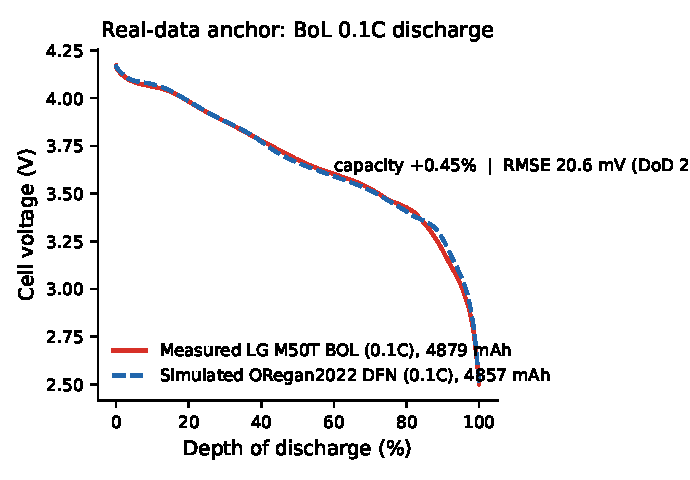
\includegraphics[width=0.78\linewidth]{figs/fig_alignment.pdf}
\caption{Real-data anchor: beginning-of-life $0.1$C discharge of a
production LG M50T 21700 cell (Imperial College dataset,
\cite{lgm50dataset2024}) versus the ORegan2022-parameterized DFN simulation
\cite{oregan2022electrochim}. Capacity agrees to $+0.45\%$; voltage RMSE
$20.6$ mV over 2--82\% depth of discharge.}
\label{fig:alignment}
\end{figure}

\subsection{Cross-Harness Portability}

The workflow's independence from any specific agent framework
(Section~3.4) is a design property of the artifact itself; its empirical
demonstration is reported here and executed in Section~5.7, so that its
results slot into Section~5 without methodological ambiguity. The design:
the identical workflow (the same declarative rule set, the same
command-line tool library, and therefore the same evaluator) runs
the same task texts (T1, a structural-bottleneck target, and T6, a
material-bottleneck target) under the same LLM and the same nominal budget setting
(300, in each harness's own turn unit) across three harnesses: the harness used throughout this paper, the
OpenAI Agents SDK, and LangChain. The measured quantities are target
attainment (checked by code, identical criteria) and audit-chain
completeness (the verifier's checks). Because the evaluator is a
command-line tool rather than harness code, the verdict mechanics are
harness-independent by design; the experiment measures whether agent
behavior under the same workflow remains faithful to the given targets when the
orchestration substrate changes, as reported in Section~5.7.
